\chapter{Descripción del problema} \label{ch:descripcion-del-problema}


\section{Definición de conceptos}\label{sec:definicion-de-conceptos}

\subsection{La arquitectura de la consola \textit{NES}}\label{subsec:la-arquitectura-mips}

La \textit{Nintendo Entertainment System}\cite{NES}, comúnmente conocida como
la \textbf{\textit{NES}}, es la segunda consola de sobremesa desarrollada por
\textit{Nintendo}.
La \textit{NES} presenta una arquitectura muy interesante:
la \textbf{unidad central de procesamiento (\textit{CPU})} es un procesador
de 8 bits basado en el famoso procesador \textbf{MOS 6502}\cite{MOS6502}.
La \textbf{unidad de procesamiento de imágenes (\textit{PPU})}\cite{PPU} está
diseñada para \delODR{utilizar}\newODR{hacer uso de} la menor memoria posible, utilizando para
\delODR{el dibujado}\newODR{dibujar} un conjunto de paletas de cuatro colores y un conjunto
de teselas.
La \textbf{unidad de procesamiento de audio (\textit{APU})}\cite{APU} presenta
cuatro canales de sonido principales: dos de pulso, uno triangular
y uno de ruido.

Gracias a su funcionamiento mediante cartuchos y que la
\textit{NES} permitía hacer operaciones \delODR{s}\newODR{d}e escritura en el cartucho,
los desarrolladores podían aumentar las capacidades de la \textit{NES} de manera sencilla,
añadiendo en el cartucho más memoria, chips de procesamiento específicos
o canales de sonido.
Estos chips reciben el nombre de \textbf{\textit{mapeadores}
o controladores de memoria}.\cite{MAPPERS}\note{Óscar: en la entrada
  bibliográfica deberías poner la fecha de consulta}.

\subsection{Carga dinámica de componentes en aplicaciones \textit{Java}}
\label{subsec:carga-dinamica-de-componentes-en-aplicaciones-java}

Un componente puede definirse como un \textbf{programa externo que modifica
el comportamiento de una aplicación principal}, añadiendo nuevas
características o modificando las ya existentes.

Existe una gran variedad de técnicas para cargar código externo
que modifique el comportamiento de una aplicación.
Muchas aplicaciones incorporan un \textbf{intérprete} para un
lenguaje de alto nivel, otras aplicaciones prefieren usar
el \textbf{propio lenguaje de programación} con el que ha sido creado.

Este es el caso de la mayoría de aplicaciones desarrolladas
en \textit{Java}\cite{JAVA_PLUGINS}.
\newODR{La máquina virtual de Java (\textit{Java Virtual Machine, o JVM})} permite \textbf{vincular y desvincular} nuevo código externo
usando las propias librerías proporcionadas por el \textit{SDK}.
Aplicaciones como \textit{Spigot}\cite{SPIGOT} o \textit{Sponge}\cite{SPONGE} aprovechan esta
tecnología para permitir que su comunidad desarrolle nuevos
componentes.
El procedimiento es sencillo: se crea una nueva clase que extienda a la
clase deseada y se indica su ruta en un pequeño archivo.
\delODR{La aplicación cargará una nueva instancia de la clase
cuando la aplicación sea lanzada que actúa de
\textbf{punto de entrada} para el componente.}
\newODR{Cuando se lance la aplicación esta cargará una nueva instancia
  de la clase, que actuará como \textbf{punto de entrada} para el componente.}

\subsection{Simuladores y emuladores}
\label{subsec:simuladores-y-emuladores}

Tanto los simuladores como los emuladores pueden definirse como un
programa de computador que imita el funcionamiento de uno o varios
componentes \textit{hardware}.
Un emulador o simulador puede imitar una arquitectura, permitiendo
ejecutar aplicaciones ajenas a la arquitectura del computador principal.

Es importante diferenciar los conceptos de \textbf{simulación}
y \textbf{emulación} a la hora de crear un programa que ejecute
código de arquitecturas externas.
La diferencia entre los simuladores y emuladores se manifiesta
en la manera en la que se implementan.

Un emulador tiene como objetivo \textbf{imitar el resultado}
que la arquitectura imitada produce al ejecutar un programa, sin tener
en cuenta el proceso interno que produce dicho resultado.
Los emuladores tienden a ser rápidos, intentando producir el resultado
de la manera más rápida y fiel posible.

Los simuladores tienen como objetivo \textbf{imitar el proceso}
que produce el resultado, \delODR{simulando}\newODR{reproduciendo el
  comportamiento de} todos los componentes de la arquitectura.
Los simuladores tienden a ser más lentos que los emuladores, pero son más
adecuados para desarrollar y depurar aplicaciones para la arquitectura
imitada sin tener el \textit{hardware} físicamente.

\subsection{\textit{JAMS}: \textit{Just Another MIPS Simulator}}
\label{subsec:jams-just-another-mips-simulator}

\textit{JAMS} es un \textbf{entorno de desarrollo integrado} especializado
en \textbf{lenguajes ensamblador} y desarrollado en el Trabajo
de Fin de Grado del Grado en Ingeniería de Computadores ligado
a este Trabajo de Fin de Grado.\note{Óscar: yo no diría ``ligado'', y
  pondría una cita bibliográfica al otro TFG}
\textit{JAMS} está desarrollado en \textit{Java}\cite{JAVA} junto
con la librería para aplicaciones gráficas \textit{JavaFX}\cite{JAVAFX}.
Por defecto, \textit{JAMS} únicamente permite desarrollar y simular
aplicaciones programadas en ensamblador \textit{MIPS32}.

\section{Descripción del problema}\label{sec:descripcion-del-problema}

\textit{JAMS}, aunque tenga una arquitectura modular y altamente
flexible, no posee la capacidad de \textbf{vincular y desvincular}
componentes, lo cual impide que otros desarrolladores expandan
las capacidades del entorno de desarrollo.

Independientemente de la capacidad de carga de componentes,
una arquitectura \textbf{nunca es completamente modificable} hasta que
se creen componentes para su aplicación: es necesario
\textbf{desarrollar un componente} de prueba que cubra
todos los aspectos del entorno de desarrollo.

La \textit{NES} es una consola muy importante para la historia
del videojuego, con una gran comunidad de desarrolladores detrás
de ella.
Sorprendentemente, no existe ningún entorno de desarrollo que permita
\textbf{desarrollar, ensamblar y simular} videojuegos de manera sencilla.
Lo más cercano que se puede encontrar son componentes
para entornos de desarrollo generales con soporte básico de edición y
ensamblaje para el procesador \textit{MOS 6502}.


\section{Objetivos}\label{sec:objetivos}

El objetivo principal de este proyecto es proporcionar a \textit{JAMS}
un \textbf{sistema de vinculación de componentes}, que permita cargar
y descargar componentes de manera rápida y sencilla, permitiendo
a los desarrolladores expandir las capacidades del entorno de desarrollo.

También es necesario \textbf{estabilizar y mejorar}
la arquitectura de \textit{JAMS}, creando un componente
de prueba que cubra todos los aspectos del entorno de desarrollo.
Este componente introducirá un \textbf{editor, ensamblador y simulador}
enfocados en la arquitectura de la consola \textit{NES}, permitiendo
desarrollar videojuegos dentro de \textit{JAMS}.

\delODR{En este apartado se detallarán diferentes objetivos.}\newODR{A
  continuación se detallarán los diferentes objetivos parciales en los
  que se ha descompuesto este objetivo principal.}

\subsection{Desarrollar un sistema de vinculación de componentes para \textit{JAMS}}
\label{subsec:desarrollar-un-sistema-de-vinculacion-de-componentes-para-jams}

Este es el \textbf{primer objetivo} que se debe superar en el transcurso de este
proyecto.
Para ello, se debe desarrollar un \textbf{vinculador de componentes} que permita
instalar y desinstalar componentes sin \textbf{tener que reiniciar la aplicación}.

\noexpand Este objetivo puede separarse en dos pasos:
\begin{itemize}
    \item Desarrollar el sistema base, que permita cargar código \textit{ByteCode}
    usando las librerías proporcionadas por el \textit{SDK} de \textit{Java}.
    \item Desarrollar un sistema de \textbf{proveedores}, permitiendo
    eliminar todos los elementos proporcionados por un componente
    cuando este \delODR{es}\newODR{sea} desinstalado por el usuario.
\end{itemize}

\subsection{Desarrollo y mejora de tecnologías relacionadas con los componentes}
\label{subsec:desarrollo-y-mejora-de-tecnologias-relacionadas-con-los-componentes}

Este objetivo se centra en desarrollar y mejorar la tecnología de \textit{JAMS}
para permitir a los componentes modificar todos los aspectos del entorno de
desarrollo de una manera rápida y sencilla.

Estas tecnologías se desarrollarán al mismo tiempo que el propio entorno
de desarrollo \textit{JAMS} y el componente de prueba, produciendo así
un código \textbf{limpio y robusto}.\note{Óscar: pero el desarrollo de
  JAMS no es parte de este proyecto, así que esto no puedes decirlo así}

\subsection{Desarrollar un entorno de desarrollo para la arquitectura \textit{NES}}
\label{subsec:desarrollar-un-entorno-de-desarrollo-para-la-arquitectura-mips32}

Para conseguir una librería robusta, se ha decidido desarrollar un componente
que proporcione a \textit{JAMS} un \textbf{editor}, \newODR{un}
\textbf{ensamblador} y \newODR{un} \textbf{simulador}
para la arquitectura de la consola \textit{NES}.
Este nuevo entorno de desarrollo debe proporcionarse \textbf{íntegramente}
mediante un componente que el usuario pueda instalar en la aplicación
principal.
Es decir, el código de \textit{JAMS} no debe proveer de ningún
tipo de tecnología específica para el desarrollo de la \textit{NES},
ni ninguna dependencia que requiera exclusivamente el componente.

Este entorno de desarrollo será muy similar al proporcionado
por \textit{JAMS} para la arquitectura \textit{MIPS32},  por lo que los
subobjetivos son muy similares:

\begin{itemize}
    \item Desarrollar un editor, un ensamblador y un simulador
    para la consola \textit{NES} usando la tecnología
    proporcionada por \textit{JAMS}.
    Estos tres componentes deben ser expandibles mediante otros componentes externos.
    \item Desarrollar diferentes herramientas que complementen las funcionalidades
    del editor, del ensamblador y del simulador.
\end{itemize}

A diferencia del entorno de desarrollo \textit{MIPS32}, \newODR{del
  que ya dispone \emph{JAMS},} el entorno
de desarrollo para la \textit{NES} sí tiene como objetivo permitir crear
código válido que se pueda ejecutar en una consola real.


\section{Metodología}\label{sec:metodologia}

\begin{figure}[h]
    \centering
    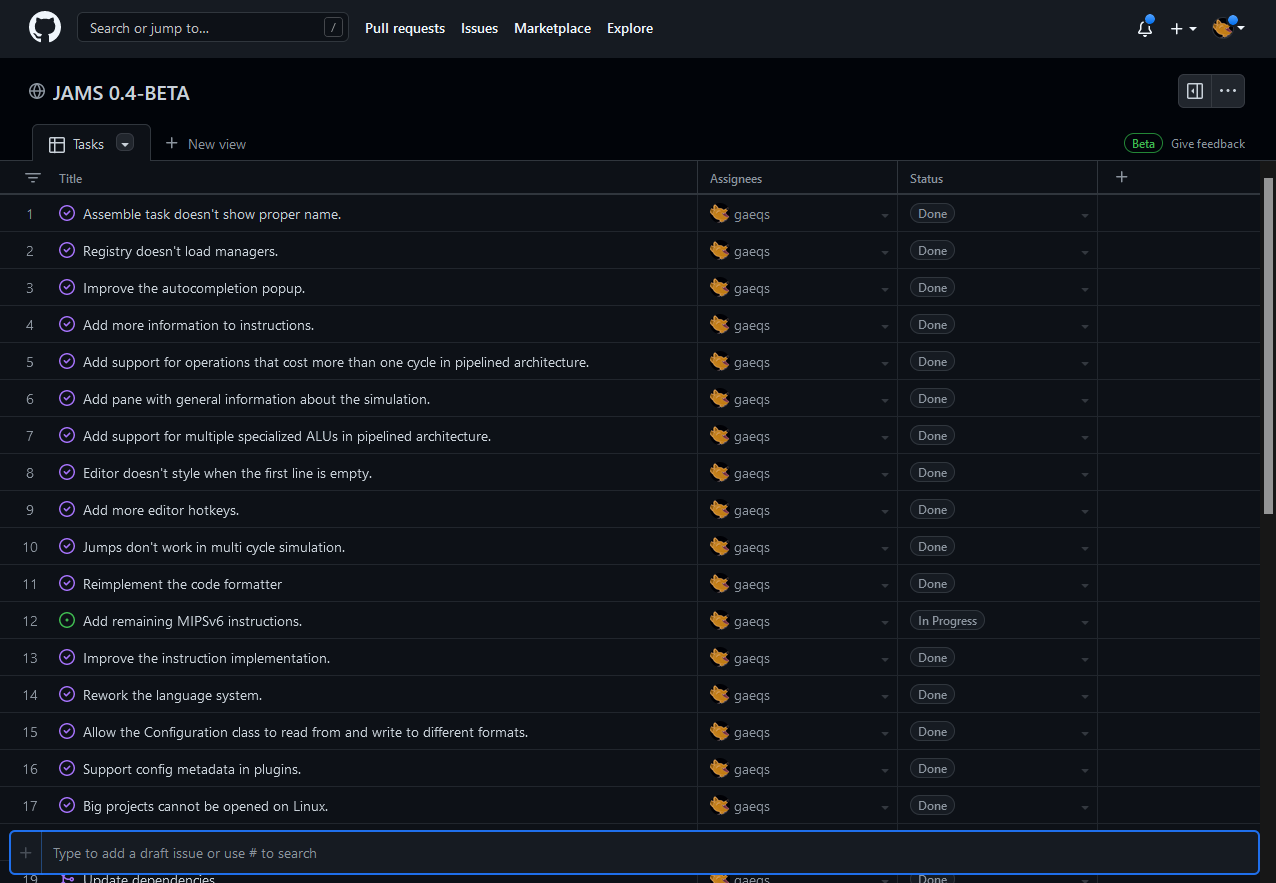
\includegraphics[width=\textwidth]{images/introduction/github}
    \caption{Proyecto de \textit{GitHub} para la versión 0.4-BETA\note{Óscar: esta figura no la referencias en el texto: por lo tanto sobra.}}
    \label{fig:introduccion-github}
\end{figure}

Debido a que la aplicación principal es muy compleja,
es muy importante marcar una metodología que permita un
desarrollo consistente, eficiente y rápido.
\textit{JAMS} ha sido desarrollado mediante una \textbf{metodología ágil},
con \textit{sprints} donde se desarrollan una serie de características claves.
Todas las características se someten a varias iteraciones donde se modifican y mejoran hasta lograr un
buen resultado.
El desarrollo de \textit{JAMS} también ha seguido un desarrollo
basado en pruebas unitarias, permitiendo mantener la calidad del
código mientras la aplicación va evolucionando.

Toda la metodología ha sido implementada mediante
las herramientas proporcionadas por \textit{GitHub}.
Los estados de las características asignadas a un \textit{sprint}
\delODR{son documentados}\newODR{se documentan} mediante proyectos.
Las acciones obligan a que las pruebas unitarias deban superarse
sin errores si se desea añadir una nueva característica a la rama principal.
Estas acciones también se emplean para generar los binarios
cuando \newODR{se supera} un \textit{sprint} \delODR{es superado} y
\newODR{se lanza} una
nueva versión de \textit{JAMS} \delODR{es lanzada}.

El componente con el entorno de desarrollo \textit{NES}
también ha seguido esta filosofía, pero a menor escala, siendo el
tiempo entre cada versión \textit{alpha} mucho menor comparado
con la aplicación principal.
